\documentclass[letterpaper,12pt]{article}
\usepackage[utf8]{inputenc}
\usepackage{fullpage}
\usepackage{courier}
\usepackage[margin=0.75in]{geometry}
\usepackage{listings}
\usepackage{color}
\usepackage{graphicx}
\usepackage[width=4in]{caption}
\usepackage{hyphenat}

% Format a sectionless paragraph
\newcommand*\unparagraph{
	\par
	\nopagebreak
	\vskip3.25ex plus1ex minus.2ex
	\noindent
}

% define extra colors
\definecolor{dkgreen}{rgb}{0,0.6,0}
\definecolor{purple}{RGB}{159,0,197}

% define the code listing format
\lstset{
	language=C++,
	basicstyle=\ttfamily,
	backgroundcolor=\color{white},
	showspaces=false,
	showstringspaces=false,
	frame=single,
	tabsize=3,
	keywordstyle=\color{purple},
	commentstyle=\color{dkgreen},
	stringstyle=\color{blue},
	escapeinside={\%*}{*)}
}

% define the title/header
\title{\Large CS 1428\\Lab 5 Sections 19 and 6} 
\author{Jared Wallace}
\date{}

\begin{document}

\maketitle

\section*{Topic}
Today we build on the conditionals that we dealt with last week by adding logical operators
which allow us to link multiple relational expressions within a single \lstinline$else$ or \lstinline$else if$.

\unparagraph{}
The 3 logical operators in C++ are: AND (\lstinline$&&$) OR (\lstinline$||$) and NOT (\lstinline$!$)

% code example here
\begin{lstlisting}[basicstyle=\footnotesize\ttfamily]

// Using and to test a closed range
if (0 <= grade && grade <= 100)
	cout << "Grade is valid";

// using or to test two open-ended ranges.  What happens if we 
//    substitute an && for the ||?
if (grade < 0 || grade > 100)
	cout << "Grade is invalid";

// negation to flip the result
if (!(grade < 0 || grade > 100))
	cout << "Grade is valid";
\end{lstlisting}

\vspace{5mm}

We also will discuss using switch statements to simplify some of the more
complex conditional blocks.

\begin{lstlisting}[basicstyle=\footnotesize\ttfamily]
// A switch statement lets us test a single variable for several
//    specific values.
switch(letterGrade) {
	case A:
	case a:
		cout << "You got the highest possible grade!" << endl;
		break;
	case B:
	case b:
		cout << "You did pretty well!" << endl;
		break;
	case C:
	case c:
		cout << "You didn't fail!" << endl;
		break;
	case F:
	case f:
		cout << "You didn't make the cut, sorry." << endl;
		break;
	default:
		cout << "Your listed grade is invalid" << endl;
		break;
}
\end{lstlisting}

\section*{Questions}
\begin{enumerate}
	\item Circle the two conditionals that are equal:
		\begin{enumerate}
				\item\lstinline$if(x < 50 || x > 150)$
				\item\lstinline$if(!(x < 50 || x > 150))$
				\item\lstinline$if(x > 50 && x < 150)$
				\item\lstinline$if(x >= 50 && x <= 150)$
		\end{enumerate}
	\item Convert the following code into a switch statement:
		\lstinputlisting[frame=none]{labexample.cpp}
\end{enumerate}

\newpage

\section*{Programing Exercise}
Write a program that first displays the following menu:

\begin{lstlisting}[frame=none,basicstyle=\footnotesize\ttfamily]
	Please select a soda:
	1. Coca-Cola
	2. Diet Coca-Cola
	3. Sprite
	4. Dr. Pepper
	Choice: 
\end{lstlisting}

After the menu is displayed get the user's input and store it into a variable named
\textbf{choice}.  Then use a switch statement to print out the message "You chose \textless soda name\textgreater".

\vspace {10mm}

For example:
\begin{lstlisting}[frame=none,basicstyle=\footnotesize\ttfamily]
	Please select a soda:
	1. Coca-Cola
	2. Diet Coca-Cola
	3. Sprite
	4. Dr. Pepper
	Choice: 4

	You chose Dr. Pepper
\end{lstlisting}

\vspace{20mm}

% Don't forget the submission instructions!
\unparagraph{} \textbf{Name your program correctly, and submit it to homework upload. Print out your source code and staple it to the back of this sheet.  Place the packet face down on my desk.}

\vspace{20mm}

% Comic at the bottom
\begin{figure}[ht!]
	\centering
	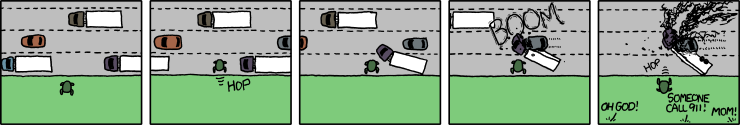
\includegraphics[width=7in]{frogger.png}
	\caption*{}I understand you and your team worked hard on this, but when we said to make it more realistic, we meant the graphics.
\end{figure}

\end{document}
